\documentclass[12pt,a4paper]{report}

\pagestyle{empty}

\usepackage[brazil]{babel}
\usepackage{graphicx,url}
\usepackage[top=2cm, bottom=2cm, left=2cm, right=2cm]{geometry}
\usepackage{hyperref}
\usepackage{cmap} % Mapear caracteres especiais no PDF
\usepackage{enumitem} % Para personalizar listas
\usepackage{amsmath} % Melhor suporte matemático
\usepackage{adjustbox} % Para ajustar o tamanho de imagens
\usepackage{float} % Para posicionar imagens

\hyphenpenalty=5000 % Evitar hifenização
\tolerance=1000     % Evitar ultrapassar margens

\begin{document}
	\begin{center}
		{\Large Universidade Federal de Uberlândia - UFU}
		
		Bacharelado em Sistemas de Informação
		
		\textbf{FACOM32504 - Redes de Computadores - 2024/2}
		
		\textbf{Arthur Fernandes - 11911BCC059}
	\end{center}
	
	\vspace{10pt}

	\begin{center}
		{\LARGE \textbf{Relatório 2 \\ \vspace{10pt} Protocolo HTTP}}
	\end{center}
	
	\vspace{10pt}
	
	\begin{figure}[ht]
		\centering
		
\includegraphics[width=0.3\textwidth]{ufu.png}
		\caption{Logo da UFU.}
		\label{fig:logoUFU1}
	\end{figure}

	\begin{enumerate}
		\item Seu navegador está executando HTTP versão 1.0, 1.1, 2 ou 3? Qual versão de HTTP o servidor está executando?
		
		\textbf{Resposta:} O navegador e o servidor estão executando a versão 1.1 do HTTP.

		\begin{figure}[H]
			\centering
			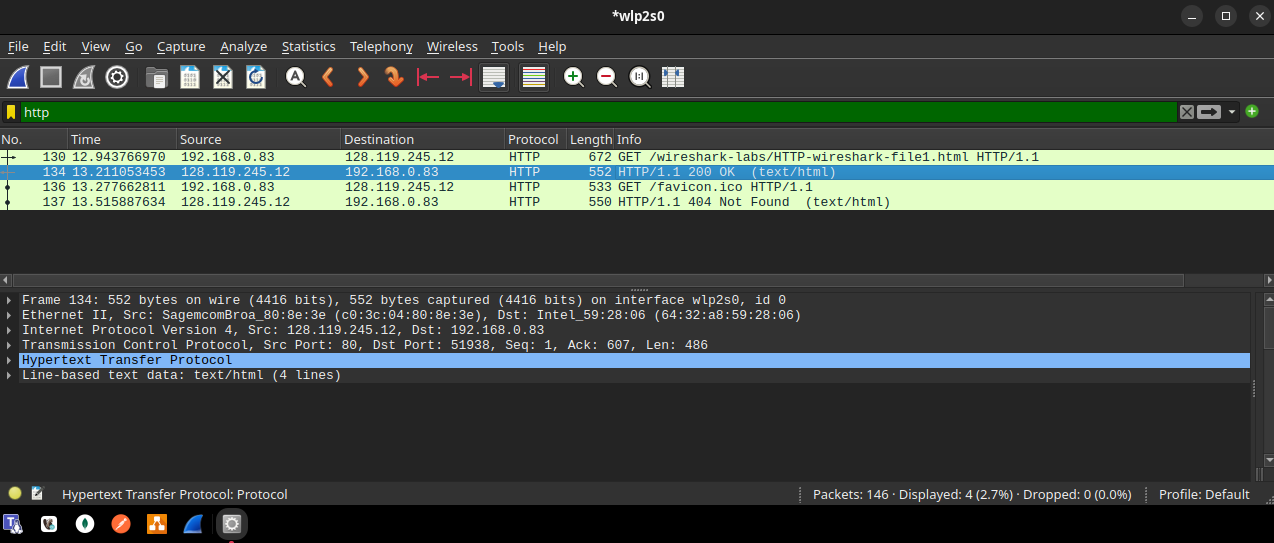
\includegraphics[width=1\textwidth]{q1.png}
			\caption{Versão do HTTP utilizada (Questão 01)}
			\label{fig:versaoHTTP}
		\end{figure}

		\item Quais idiomas (se houver) seu navegador indica que pode aceitar para o servidor?
		
		\textbf{Resposta:} O navegador indica que aceita os idiomas inglês e português.

		\begin{figure}[H]
			\centering
			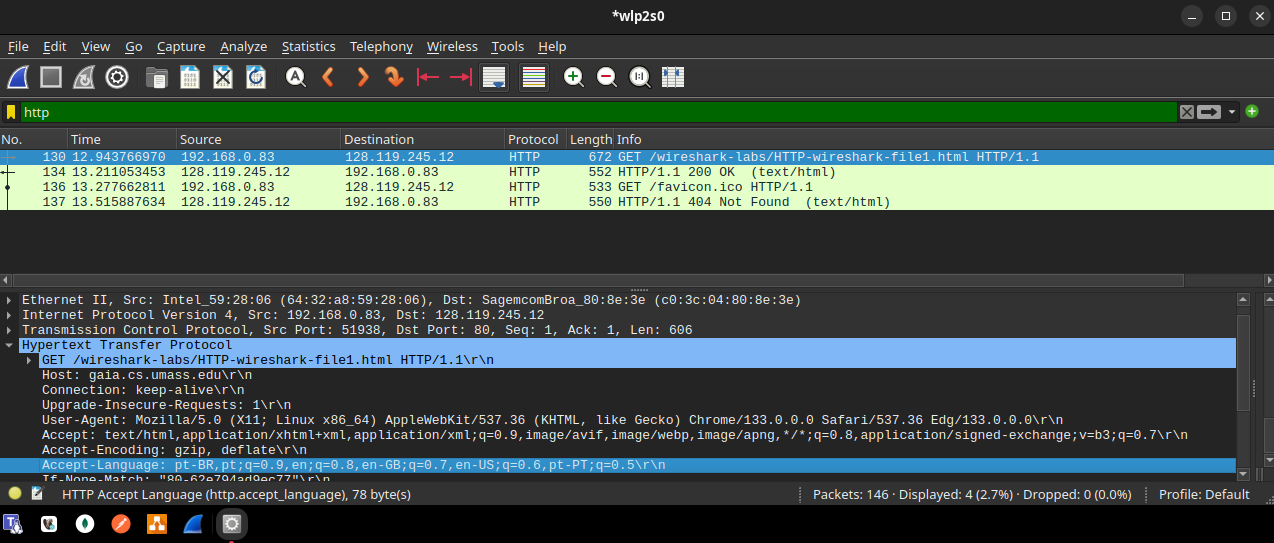
\includegraphics[width=1\textwidth]{q2.png}
			\caption{Idiomas aceitos pelo navegador (Questão 02)}
			\label{fig:idiomasAceitos}
		\end{figure}

		\item Qual é o endereço IP do seu computador? Do servidor gaia.cs.umass.edu?
		
		\textbf{Resposta:} O endereço IP do meu computador é 192.168.0.83. O endereço IP do servidor gaia.cs.umass.edu é 128.119.245.12. É possível ver nas imagens das questões anteriores.

		\item Qual é o código de status retornado do servidor para o seu navegador?
		
		\textbf{Resposta:} Para a requisição do arquivo /wireshark-labs/HTTP-wireshark-file1.html o servidor respondeu com 200 OK. Para a requisição do favicon (/favicon.ico) o servidor respondeu com 404 Not Found. É possível ver nas imagens das questões anteriores.

		\item Quando o arquivo HTML que você está recuperando foi modificado pela última vez no servidor?

		\textbf{Resposta:} O arquivo foi modificado pela última vez no servidor em 20 de fevereiro de 2025.

		\begin{figure}[H]
			\centering
			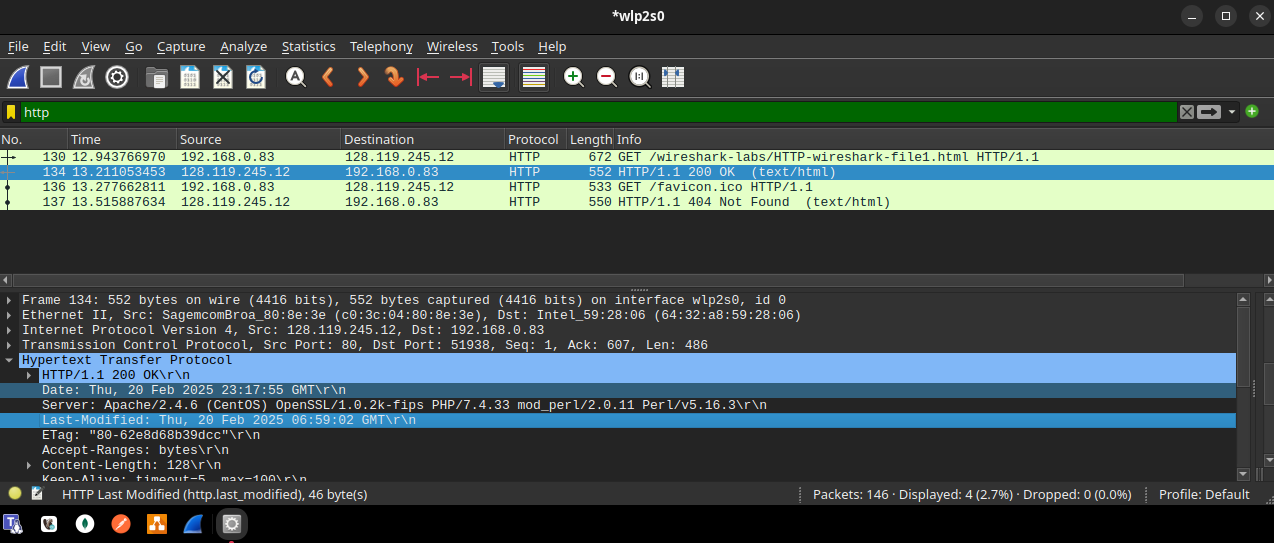
\includegraphics[width=0.9\textwidth]{q5.png}
			\caption{Data da última modificação do arquivo (Questão 05)}
			\label{fig:dataUltimaModificacao}
		\end{figure}

		\item Quantos bytes de conteúdo estão sendo retornados ao seu navegador?
		
		\textbf{Resposta:} 128 bytes.

		\begin{figure}[H]
			\centering
			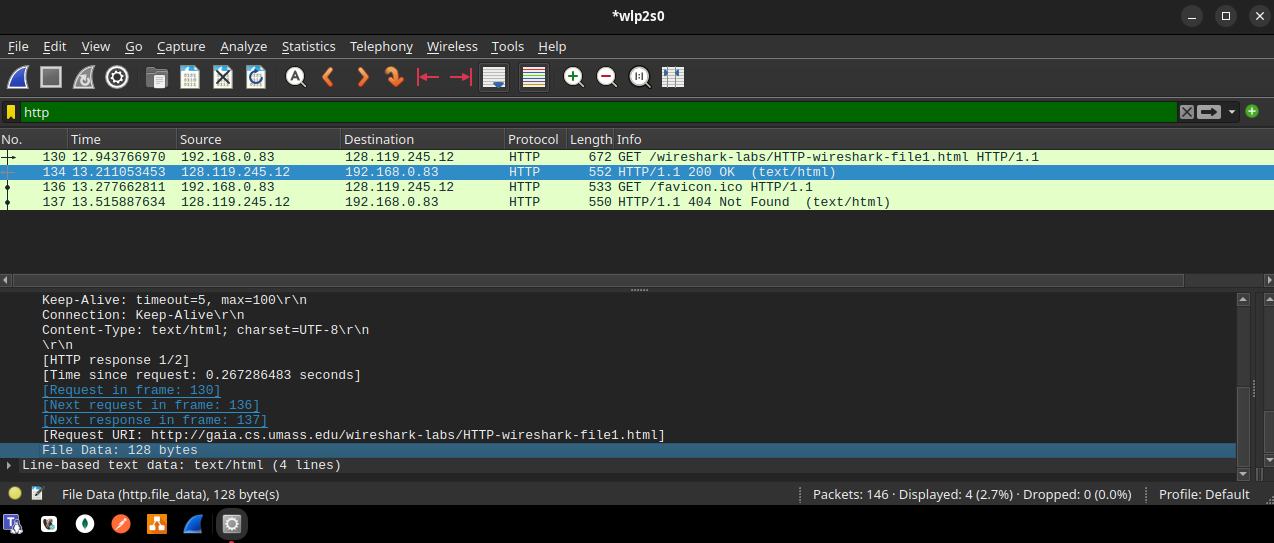
\includegraphics[width=1\textwidth]{q6.png}
			\caption{Tamanho conteúdo retornado (Questão 06)}
			\label{fig:tamanhoConteudo}
		\end{figure}

		\item Ao inspecionar os dados brutos na janela de conteúdo do pacote, você vê algum cabeçalho nos dados que não são exibidos na janela de listagem de pacotes? Se sim, escreva um.

		\textbf{Resposta:} Sim. Apache/2.4.6 (CentOS)

		\item Inspecione o conteúdo da primeira solicitação HTTP GET de seu navegador para o servidor. Você vê uma linha “IF-MODIFIED-SINCE” no HTTP GET?

		\textbf{Resposta:} Sim, ele contém: If-Modified-Since: Wed, 19 Feb 2025 06:59:01 GMT.

		\item Inspecione o conteúdo da resposta do servidor. O servidor retornou explicitamente o conteúdo do arquivo? Como você sabe?

		\textbf{Resposta:} Sim, o servidor retornou explicitamente o conteúdo do arquivo HTML solicitado. Pois o código de status é 200 OK

		\item Agora inspecione o conteúdo da segunda solicitação HTTP GET de seu navegador para o servidor. Você vê uma linha “IF-MODIFIED-SINCE:” no HTTP GET? Em caso afirmativo, quais informações seguem o cabeçalho “IF-MODIFIED-SINCE:”?

		\textbf{Resposta:} Dessa vez não consegui encontrar a linha “IF-MODIFIED-SINCE” no HTTP GET.

		\item Qual é o código de status HTTP e a frase retornada do servidor em resposta a este segundo HTTP GET? O servidor retornou explicitamente o conteúdo do arquivo? Explique.

		\textbf{Resposta:} A segunda requisição (GET /favicon.ico) falhou, pois obteve código 404 Not Found. Logo, o servidor não retornou explicitamente o conteúdo do arquivo.

		\item Quantas mensagens de solicitação HTTP GET seu navegador enviou? Qual número de pacote no rastreamento contém a mensagem GET para a Declaração de Direitos (Bill of Rights)?

		\textbf{Resposta:} Apenas duas mensagens de solicitação HTTP GET foram enviadas.

		\begin{figure}[H]
			\centering
			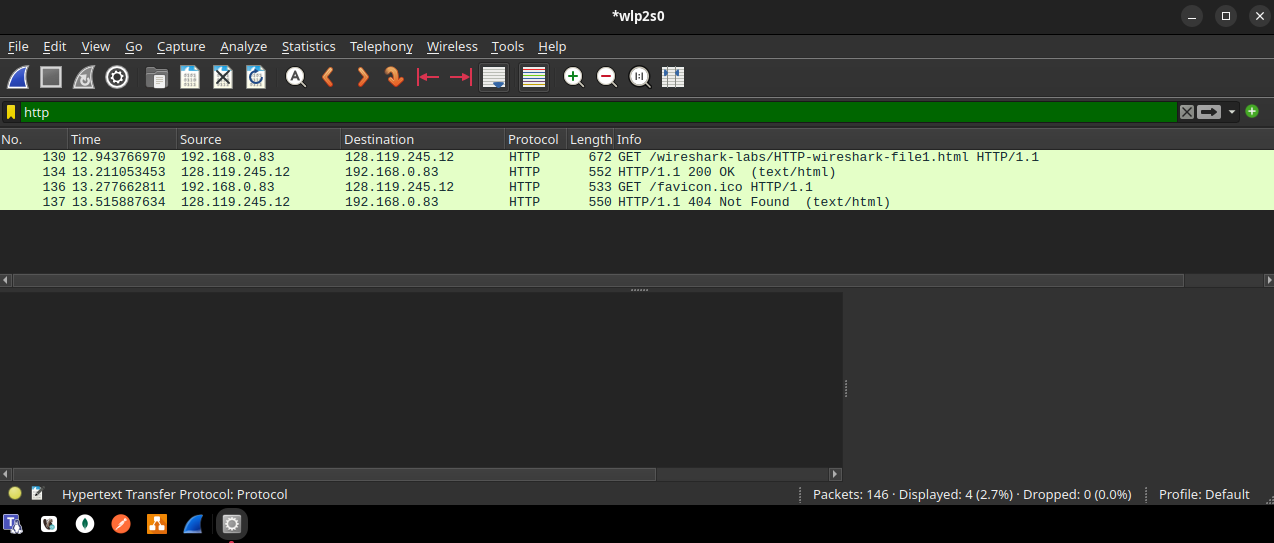
\includegraphics[width=1\textwidth]{q12.png}
			\caption{Número de pacote da mensagem GET (Questão 12)}
			\label{fig:numeroPacoteGET}
		\end{figure}

		\item Qual número de pacote no rastreamento contém o código de status e a frase associada à resposta à solicitação HTTP GET?

		\textbf{Resposta:} Apenas 02 pacotes.

		\item Qual é o código de status e a frase na resposta?
		
		\textbf{Resposta:} Status 200 OK e outro 404 Not Found.	

		\item Quantos segmentos TCP contendo dados foram necessários para transportar a única resposta HTTP e o texto da Declaração de Direitos?

		\textbf{Resposta:} Infelizmente não consegui encontrar a resposta para essa questão.

		\item Quantas mensagens de solicitação HTTP GET seu navegador enviou? Para quais endereços de Internet essas solicitações GET foram enviadas?

		\textbf{Resposta:} Apenas duas. Endereço destino: 128.119.245.12

		\item Você pode dizer se o seu navegador baixou as duas imagens em série ou se elas foram baixadas dos dois sites em paralelo? Explique.

		\textbf{Resposta:} As imagens foram baixadas em série, pois o navegador só enviou a segunda requisição após a primeira ter sido respondida.

		\item Qual é a resposta do servidor (código de status e frase) em resposta à mensagem HTTP GET inicial do seu navegador?

		\textbf{Resposta:} Status 200 OK

		\item Quando o seu navegador envia a mensagem HTTP GET pela segunda vez, qual novo campo é incluído na mensagem HTTP GET?

		\textbf{Resposta:} If-Modified-Since
		
	\end{enumerate} 

\end{document}
